Накопление спектра производим в течение 600 секунд. Спектры представим на рис.
\ref{img::Na}-\ref{img::Eu}. Проведём измерение фона (см. рис. \ref{img::Back}) и убедимся, что интенсивность его
спектра много меньше интенсивности спектра исследуемых образцов; также в спектре
фона нет пиков.


\begin{figure}
\begin{center}
  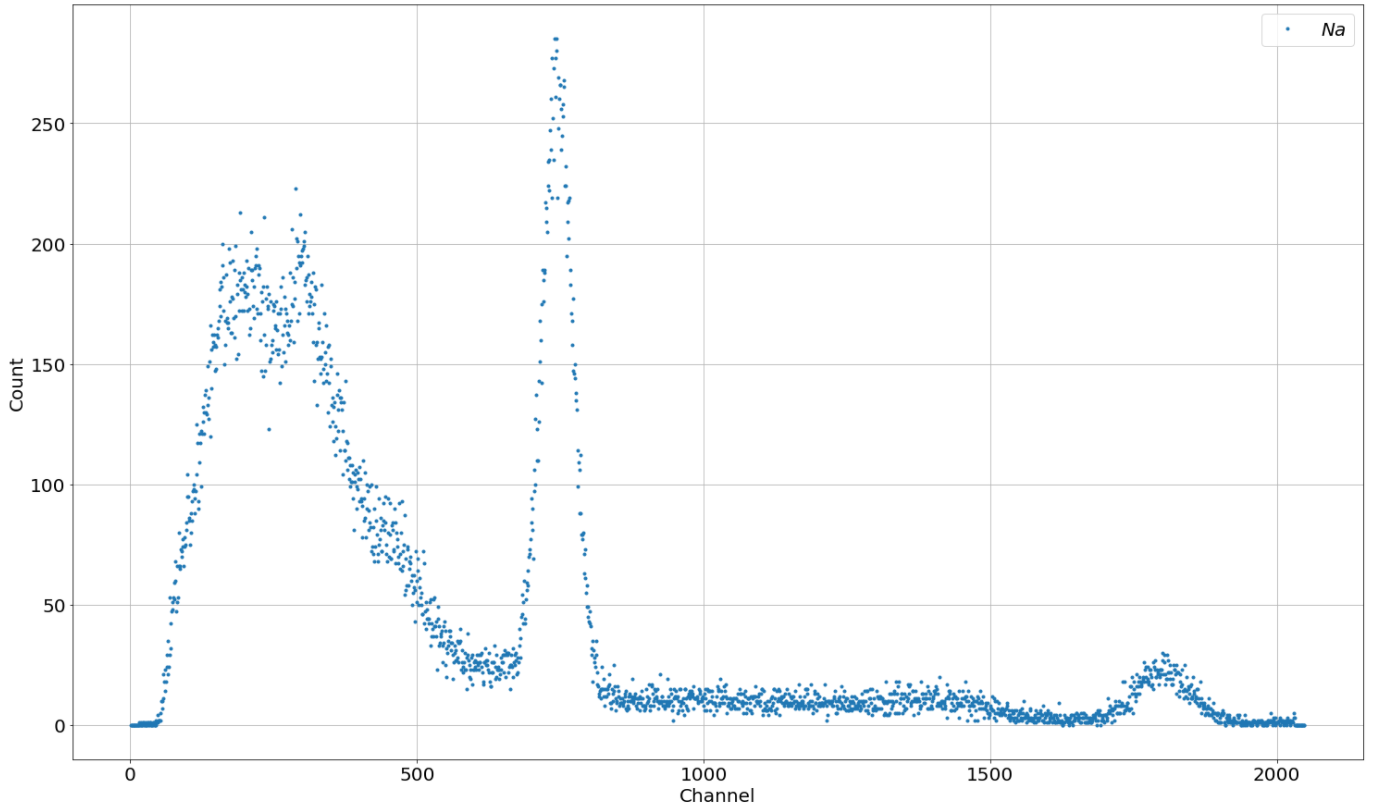
\includegraphics[width=0.8\linewidth]{Na.png}
  \caption{Спектр ${}^{22}{\text{Na}}$}
  \label{img::Na}
  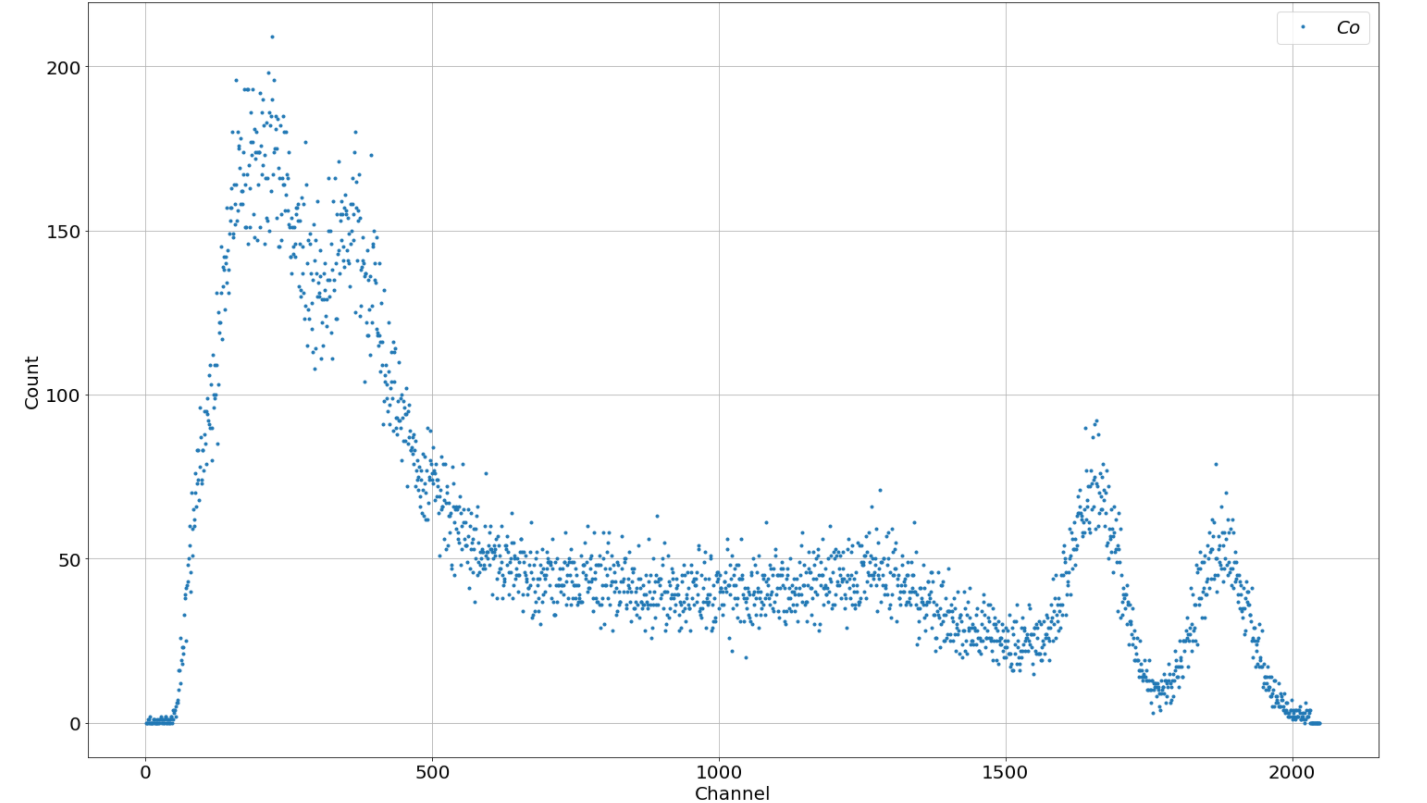
\includegraphics[width=0.8\linewidth]{Co.png}
  \caption{Спектр ${}^{60}{\text{Co}}$}
  \label{img::Co}
\end{center}
\end{figure}

\begin{figure}
\begin{center}
  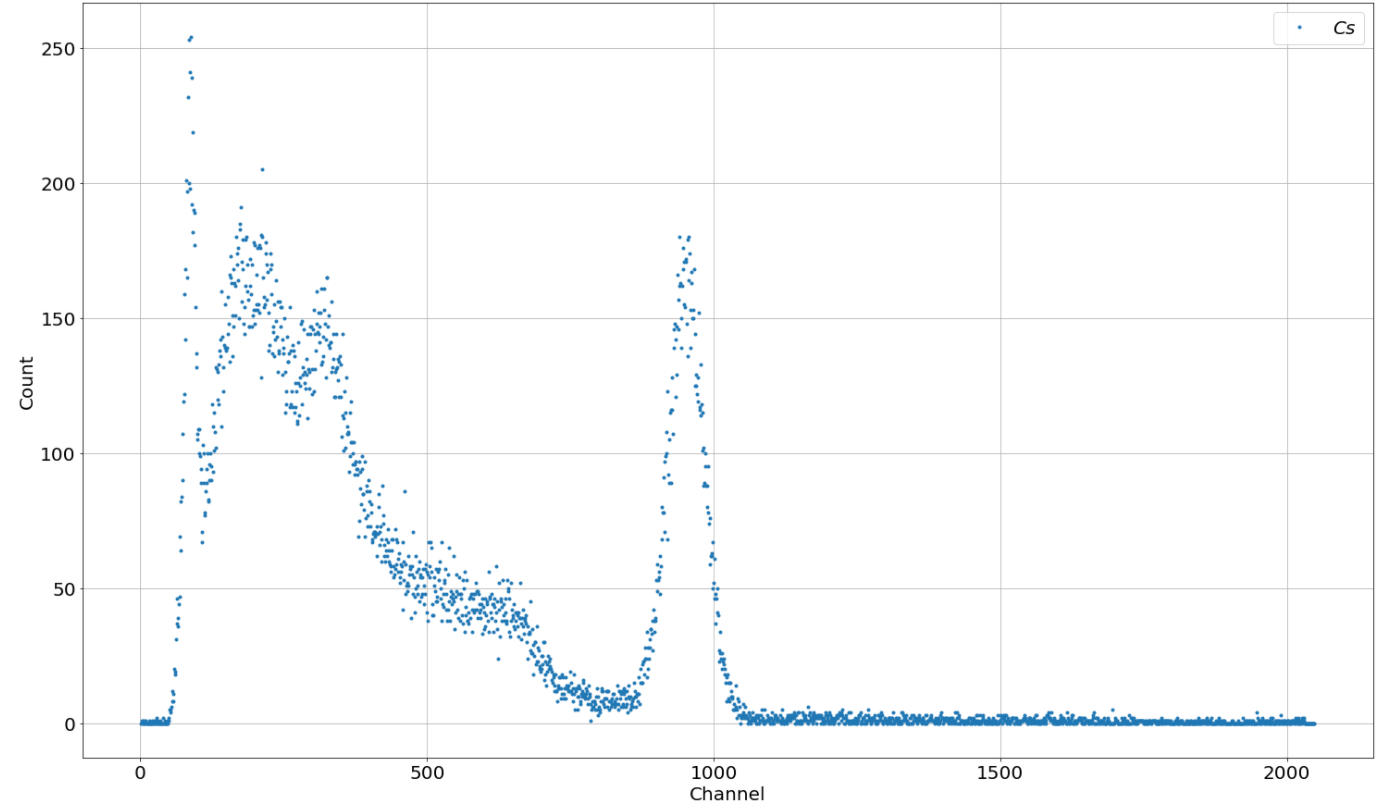
\includegraphics[width=0.8\linewidth]{Cs.png}
  \caption{Спектр ${}^{137}{\text{Cs}}$}
  \label{img::Cs}
  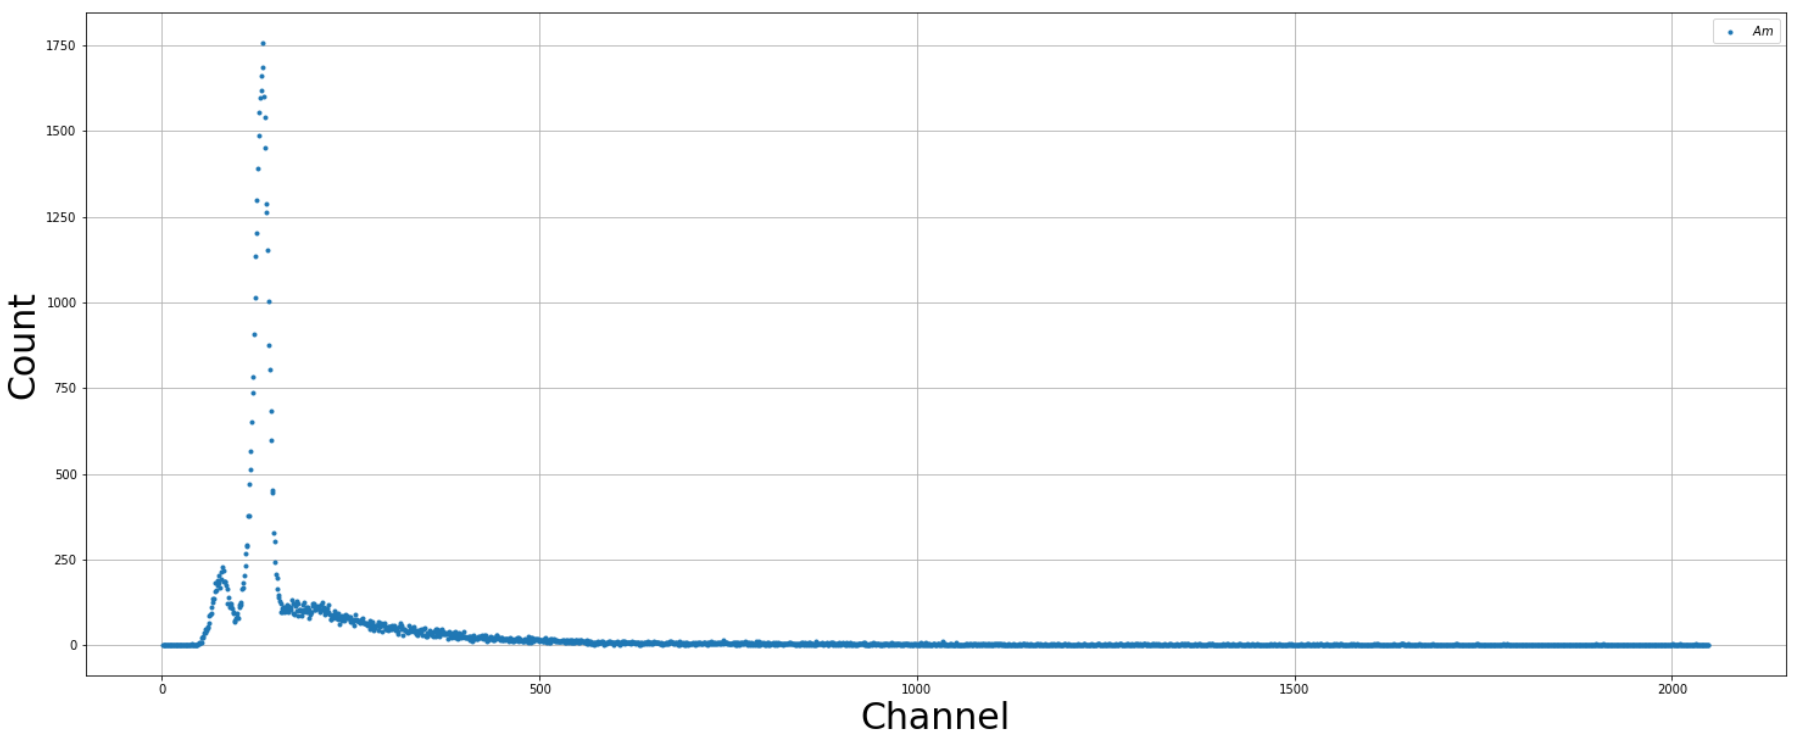
\includegraphics[width=0.8\linewidth]{Am.png}
  \caption{Спектр ${}^{241}{\text{Am}}$}
  \label{img::Am}
\end{center}
\end{figure}

\begin{figure}
\begin{center}
  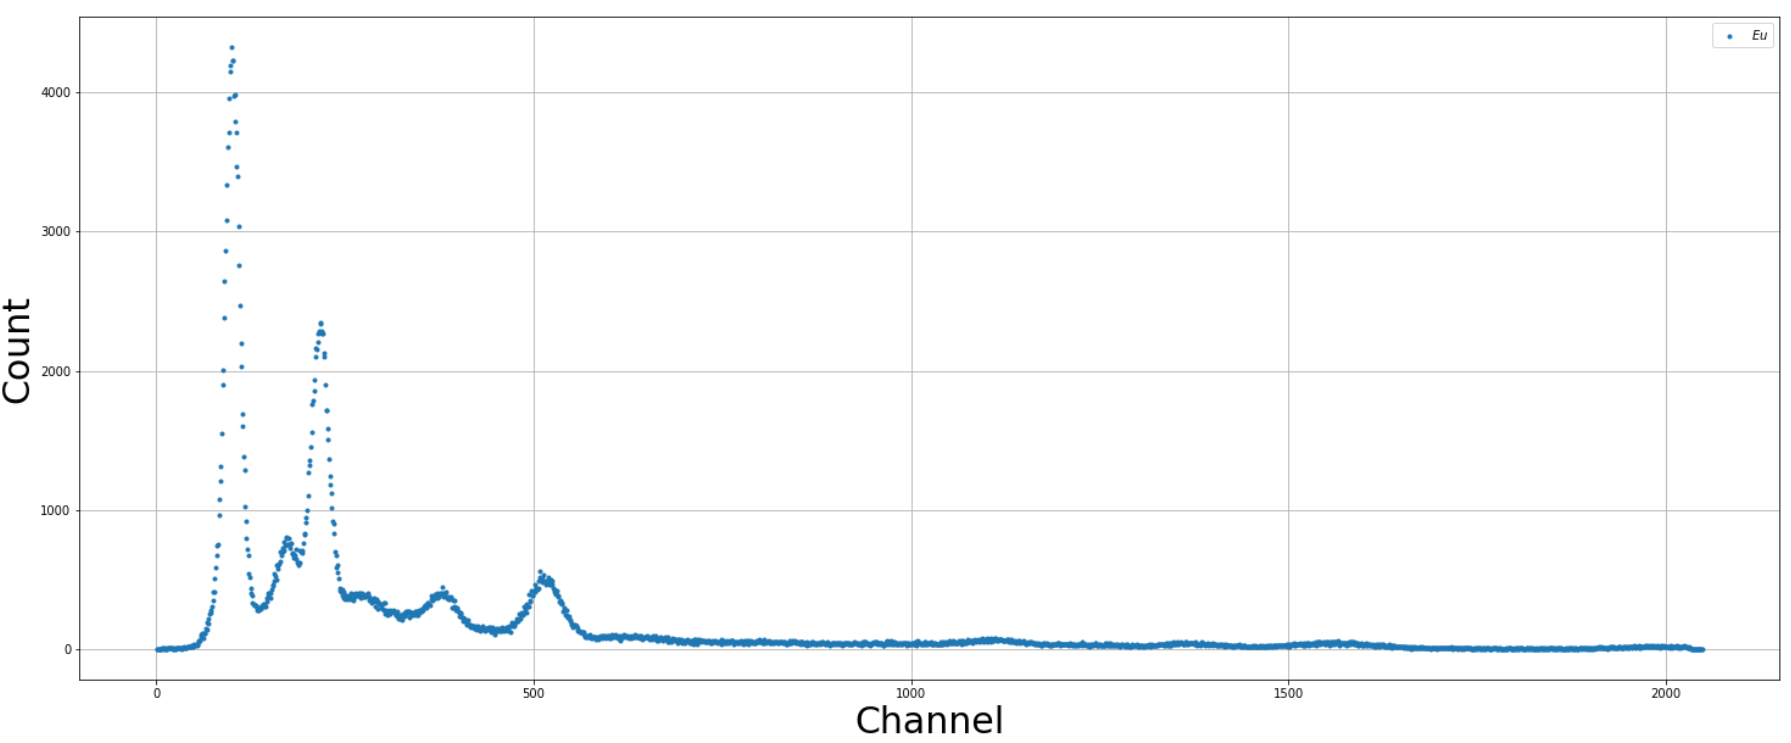
\includegraphics[width=0.8\linewidth]{Eu.png}
  \caption{Спектр ${}^{152}{\text{Eu}}$}
  \label{img::Eu}
  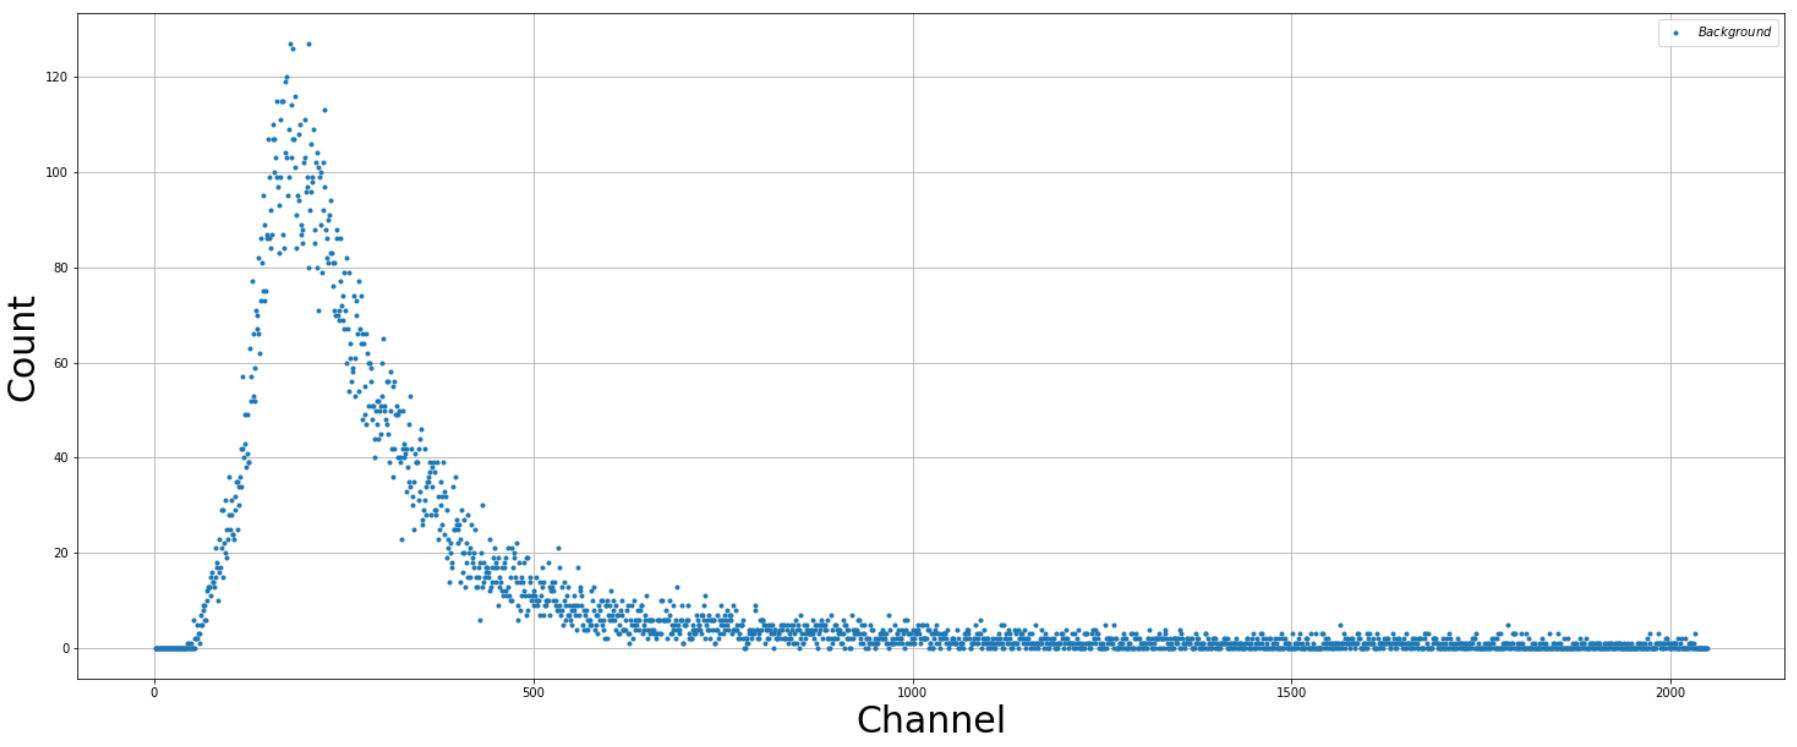
\includegraphics[width=0.8\linewidth]{Back.png}
  \caption{Спектр фона}
  \label{img::Back}
\end{center}
\end{figure}
Используя известные значения пиков в спектрах натрия и цезия, построим
калибровочный график соответствия номера канала определённому значению энергии
(рис. \ref{img::calibrate}).

\begin{figure}[h!]
  \centering
  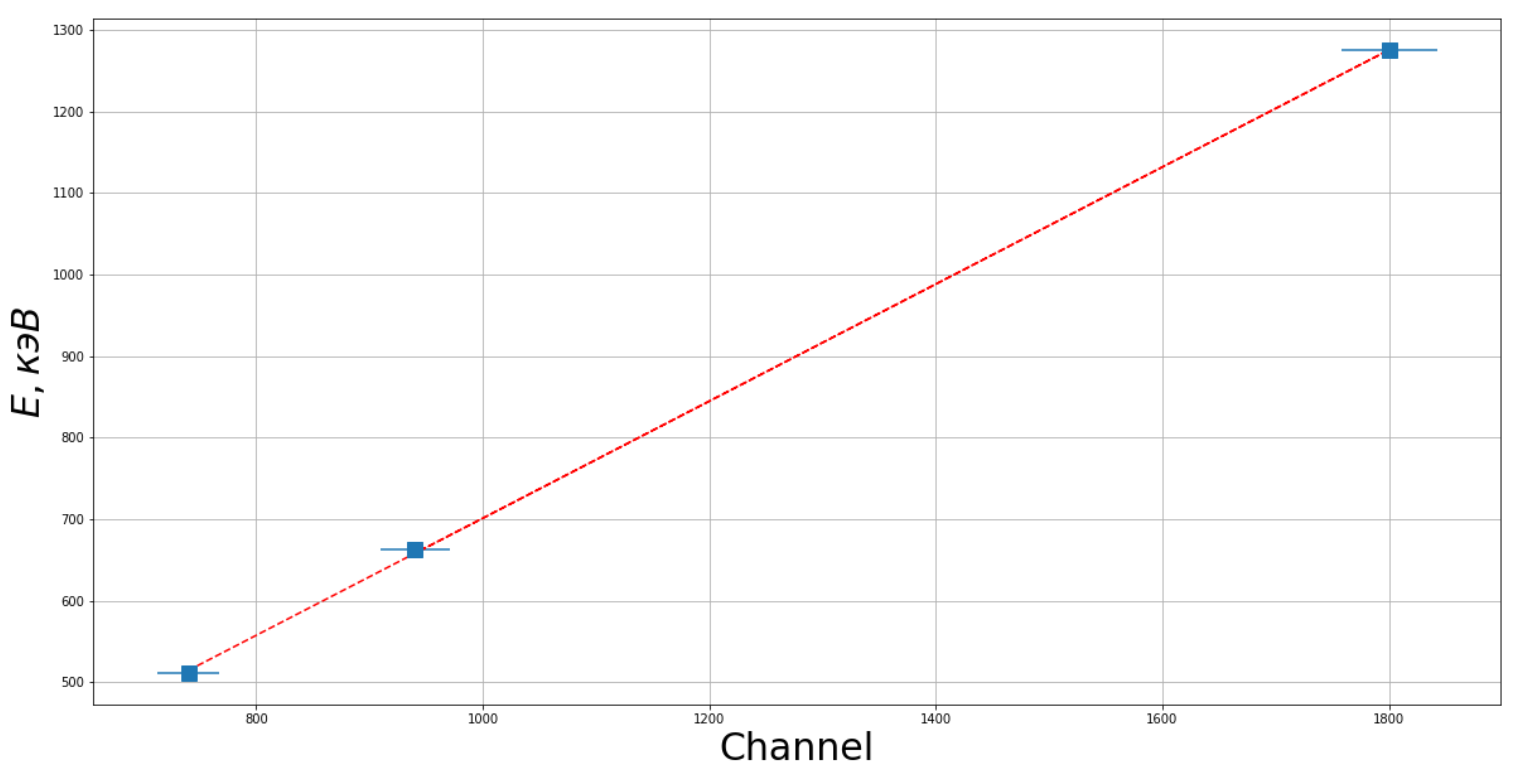
\includegraphics[width=0.8\linewidth]{channel_from_energy.png}
  \caption{Калибровочный график}
  \label{img::calibrate}
  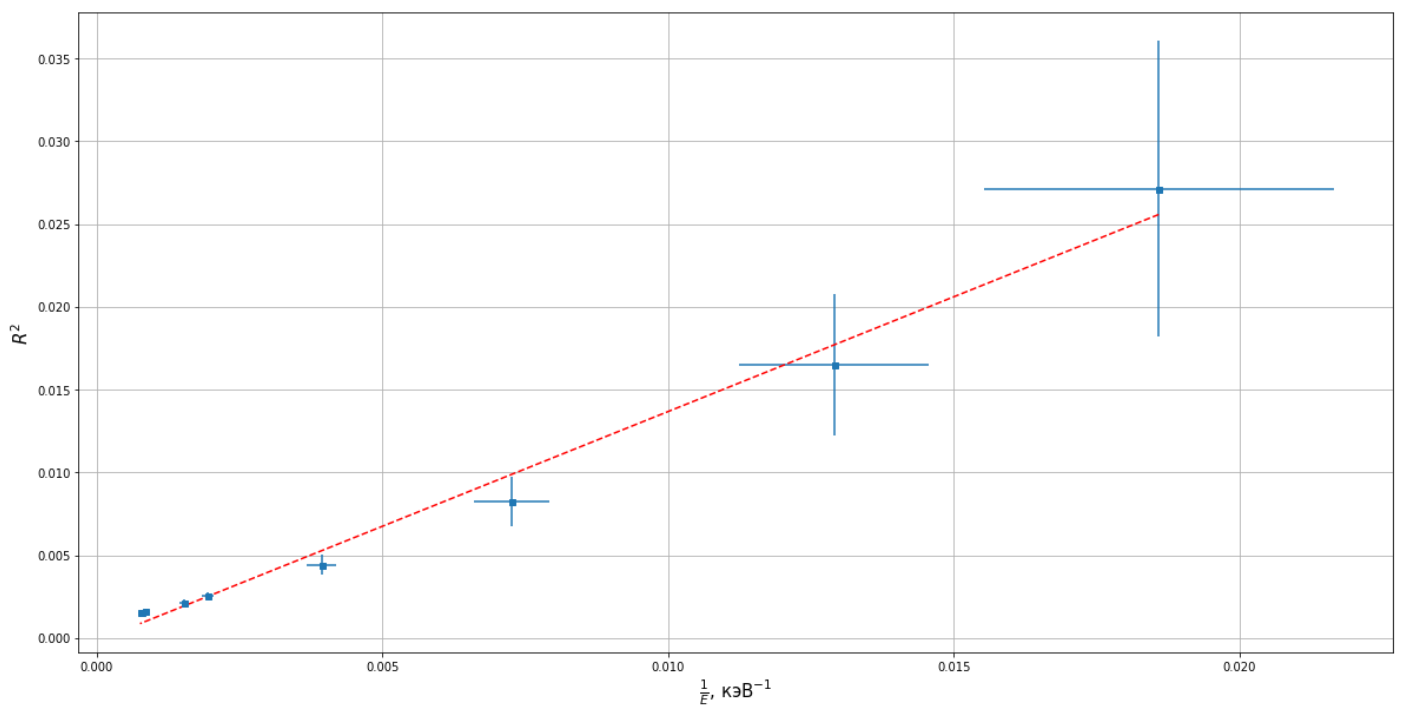
\includegraphics[width=0.8\linewidth]{r_sq_from_e.png}
  \caption{График зависимости $R^2 = f(\frac{1}{E})$}
  \label{img::Rsqrt}
\end{figure}

Получаем уравнение для перехода от номера канала к значению энергии в кэВ:
\begin{center}
    $E = (0.718 \pm 0.004)N_i - (17 \pm 5)$
\end{center}

Используя калибровочный график, определим для всех остальных источников значения
энергии пиков полного поглощения $E_i$, их ширины на половине высоты $\Delta
E_i$ и энергетическое разрешение $R_i$. Результаты занесём в таблицу \ref{tab:my_label}.

\begin{table}[h]
\begin{center}
  \caption{Пики полного поглощения различных образцов}
  \label{tab:my_label}
  \import{./src/}{picks.tex}
\end{center}
\end{table}

Проверим зависимость \eqref{eq::Rsqrt}. Для этого построим график зависимости $R^2 = f(\frac{1}{E})$
(рис. 10). Наблюдается линейная зависимость, что согласуется с теоретической зависимостью. Из-за неточностей в определении
полуширины пиков точки не лежат на одной прямой.

Определим энергии края комптоновского поглощения для образцов $^{22}$Na,
$^{137}$Cs, $^{60}$Co, а также вычислим теоретические значения этих энергий по
формуле \eqref{eq::Ehw}. Построим график, по одной оси отложив экспериментальные
значения, а по другой -- теоретические (\ref{img::th_exp}). Вычислим коэффициент
наклона прямой $a = 1.04 \pm 0.06$ --  с учётом погрешности коэффициент наклона
совпадет с единицей, что говорит о согласованности с теорией.

\begin{figure}[h!]
  \centering
  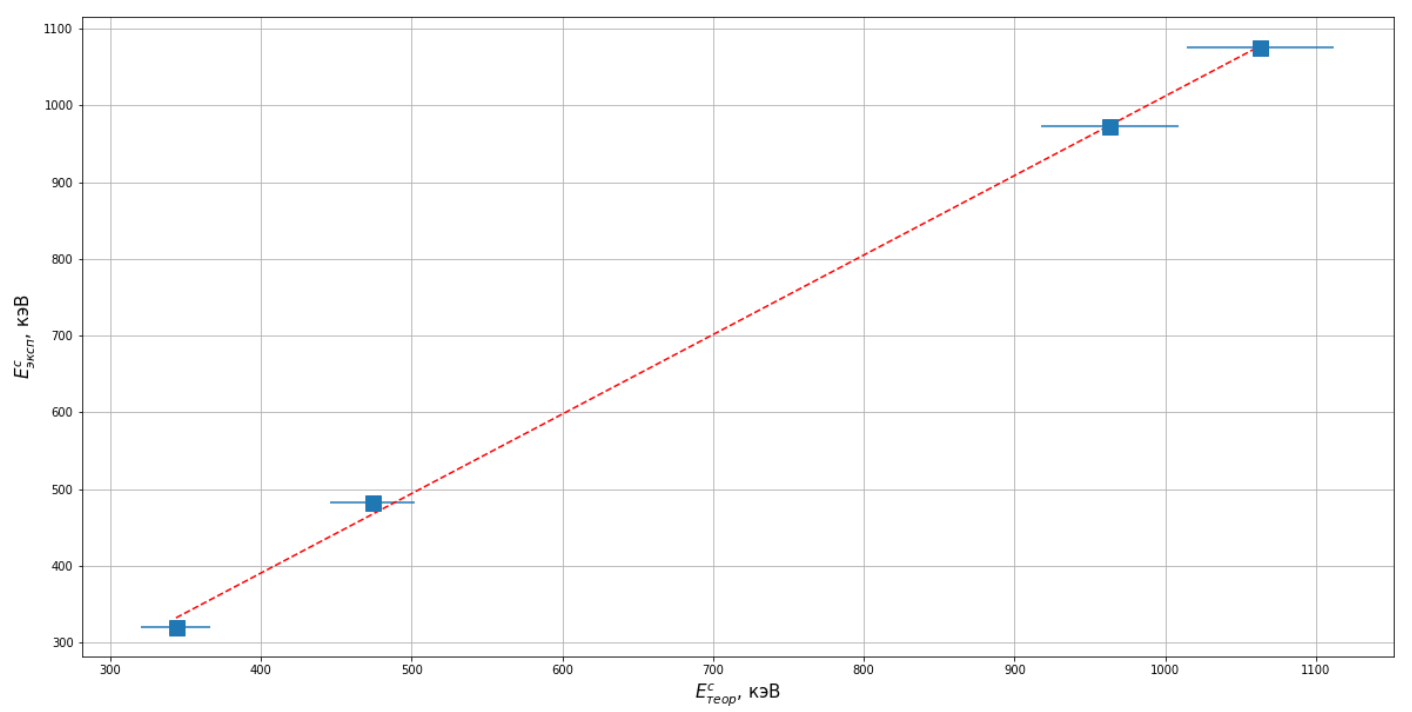
\includegraphics[width=0.8\linewidth]{th_from_exp.png}
  \caption{Сравнение теоретических и экспериментальных энергий края К.П.}
  \label{img::th_exp}
\end{figure}

\begin{table}[h!]
  \begin{center}
    \caption{Комптоновские спектры}
    \import{./src/}{comp.tex}
  \end{center}
\end{table}

В спектрах, где наблюдаются пики обратного рассеяния, определим энергии этих
пиков и построим график зависимости энергии пика обратного рассеяния от энергии.
Также по формуле \eqref{eq::E_rev} построим теоретический график этой
зависимости (\ref{img::e_obr}).
По графику видно, что характер зависимости достаточно близок к теории.
\begin{table}[h!]
  \centering
  \caption{Пики прямого поглощения}
  \begin{tabular}{| c | c | c | c | c | c | c |}
\hline
Элемент & $N_i$ & $\sigma_{N_i}$ & $E_i$, кэВ & $\sigma_{E_i}$, кэВ & $R_i$ & $\sigma_{R_i}$\\
\hline
$^{22}\text{Na}$ & $740$ & $27$ & $742$ & $31$ & $0.042$ & $0.002$\\
\hline
$^{22}\text{Na}$ & $1800$ & $42$ & $1840$ & $54$ & $0.0298$ & $0.0009$\\
\hline
$^{137}\text{Cs}$ & $940$ & $30$ & $949$ & $36$ & $0.038$ & $0.001$\\
\hline
$^{60}\text{Co}$ & $1657$ & $40$ & $1692$ & $51$ & $0.0306$ & $0.0009$\\
\hline
$^{60}\text{Co}$ & $1865$ & $43$ & $1907$ & $56$ & $0.0294$ & $0.0009$\\
\hline
$^{241}\text{Am}$ & $132$ & $11$ & $113$ & $13$ & $0.11$ & $0.01$\\
\hline
$^{152}\text{Eu}$ & $99$ & $9$ & $79$ & $11$ & $0.14$ & $0.02$\\
\hline
$^{152}\text{Eu}$ & $216$ & $14$ & $200$ & $16$ & $0.081$ & $0.007$\\
\hline
$^{152}\text{Eu}$ & $378$ & $19$ & $368$ & $21$ & $0.059$ & $0.003$\\
\hline
\end{tabular}

\end{table}


\begin{figure}[h!]
  \centering
  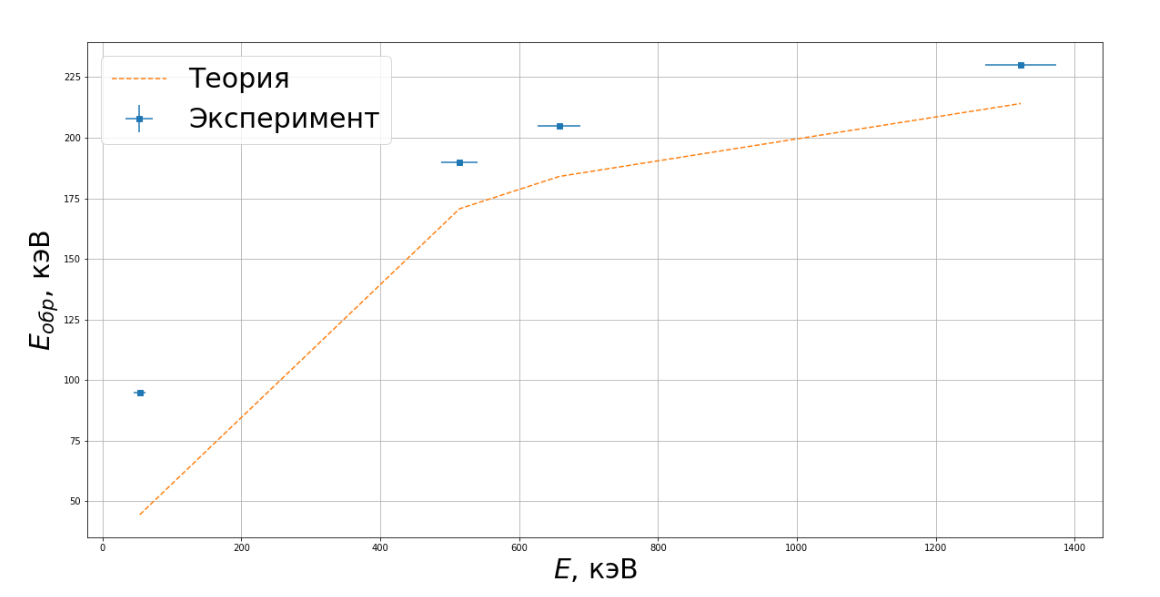
\includegraphics[width=0.8\linewidth]{e_obr.png}
  \caption{Сравнение теоретических и экспериментальных энергий обратного рассеяния}
  \label{img::e_obr}
\end{figure}

\begin{table}[h!]
  \centering
  \caption{Пики обратного рассеяния}
  \begin{tabular}{| c | c | c | c | c |}
\hline
$$ & $E_i$ & $\sigma_{E_i}$ & $E_{обр}$ & $\sigma_{E_{обр}}$\\
\hline
$^{152}\text{Eu}$ & $79.3$ & $11.5$ & $95$ & $0.1$\\
\hline
$^{22}\text{Na}$ & $742.9$ & $31.5$ & $190$ & $0.1$\\
\hline
$^{137}\text{Cs}$ & $949.9$ & $36.3$ & $205$ & $0.1$\\
\hline
$^{60}\text{Co}$ & $1907.4$ & $56.1$ & $230$ & $0.1$\\
\hline
\end{tabular}

\end{table}

Вычислим энергию наблюдаемого характеристического излучения из защитного слоя
свинца. Для этого обратим внимание на графики Цезия \ref{img::Cs}, Кобальта
\ref{img::Co}, Натрия \ref{img::Na} и Европия \ref{img::Eu}.
На этих графиках заметен всплеск на энергиях $\approx 120$ кэВ.

Зная, что форма импульсов на ФЭУ определяется выражением:
\[
  U(t) = \text{const} \cdot \e^{-\frac{t}{RC}}
  \left(1 - \e^{ - \frac{t}{\tau_0}}\right)
\]
Пронаблюдаем на осциллографе изображение импульсов с ФЭУ. По переднему фронту
оценим величину $\tau_0 \simeq 0.6$ мкс как время за которое амплитуда
увеличивается в $1 + \frac{1}{\e}$ раз. По заднему фронту оценим $RC \simeq 35$ мкс как время
за которое амплитуда уменьшается в $\e$ раз.
Данный метод оценки следует из того факта, что в начале импульса,
когда время мало, выражение $U(t)$ растёт засчёт $\left(1 - \e^{ - \frac{t}{\tau_0}}\right)$,
со временем рост замедляется, и эта часть медленно стремиться к $1$, в то время как множитель
$\e^{-\frac{t}{RC}}$ всё уменьшается, что и вызывает спад функции в конце.

\section{Вывод}

В ходе работы были получены спектры гамма излучений для образцов
$^{22}$Na, $^{127}$Cs, $^{60}$Co, $^{241}$Am и $^{152}$Eu.
Для определения энергий в спектре был построен калибровочный график,
по которому была установлена зависимость
\[
  E = a \cdot  N_i + b, \quad
  a = 0.718 \pm 0.004 \: \text{кэВ}, \:
  b = - 17 \pm 5 \:\text{кэВ}
\]
Также был проверен закон $R = \frac{\text{const}}{\sqrt{E}}$.
Построенный график зависимости $R^2 = f(1/E)$ (рис. \ref{img::Rsqrt})
показывает, что зависимость близка к теоретической.

Были исследованы пики полного поглощения и обратного рассеяния
в первом случае, построением графика теоретических значений от экспериментальных
(рис. \ref{img::th_exp}), было замечено сходство теории и практики
так как коэффициент наклона графика получился
$a = 1.04 \pm 0.06$, что с учётом погрешности совпадает с $1$.
Во втором случае, было построено одновременно теоретическая и экспериментальная
зависимости (рис. \ref{img::e_obr}), исходя из вида графика, замечено,
что характер зависимости экспериментальных данных близок к теоретической.

Была проведена оценка характеристического излучения из защитного слоя
свинца $\approx 120$ кэВ. А также проведена оценка констант
затухания и нарастания импульса ФЭУ
$RC \simeq 35$ мкс,
$\tau_0 \simeq 0.6$ мкс.